\documentclass[10pt,a4paper]{article}
\usepackage[margin=1.7cm]{geometry}
\usepackage{amsmath,amssymb}
\usepackage{booktabs}
\usepackage{array}
\usepackage{graphicx}
\usepackage{caption}
\usepackage{subcaption}
\usepackage[hidelinks]{hyperref}
\usepackage{enumitem}
\usepackage{titlesec}
\usepackage{xcolor}
\setlist{nosep,leftmargin=1.2em}
\titlespacing*{\section}{0pt}{6pt}{3pt}
\titlespacing*{\subsection}{0pt}{4pt}{2pt}
\captionsetup{font=small,skip=3pt}
\setlength{\parskip}{2pt}
\setlength{\parindent}{0pt}
\setlength{\abovedisplayskip}{3pt}
\setlength{\belowdisplayskip}{3pt}
\newcommand{\repo}{https://github.com/s-aura-bhhh/Air-quality-analysis}
\newcommand{\nb}[2]{\href{\repo/blob/main/notebooks/#1}{\texttt{\color{blue!60!black}#2}}}

\title{\vspace{-1.2cm}\textbf{Air Quality in Indian Cities: Prediction and Profiling}\\[2pt]
\large MA515 (Foundations of Data Science) -- Group Project Report}
\author{Arahana Garg (2024MCB1261) \and Kushagra Gupta (2024MCB1299) \and Saurabh Sharma (2024MCB1311) \and Manish Kumar Chatakunda (2024MCB1302)}
\date{\small Code and data: \url{\repo}}

\begin{document}
\maketitle
\vspace{-0.4cm}

%-------------------------------------------------------------
\section{Introduction and problem formulation}
Air pollution is one of India's largest public-health risks. The Central Pollution Control Board (CPCB) reports daily pollutant concentrations and an Air Quality Index (AQI) for many cities. Health warnings are issued when the AQI is \emph{Poor} or worse ($>200$). We ask whether such days can be anticipated, what drives them, and how cities differ.

\textbf{Research questions.}
\begin{itemize}
\item \textbf{RQ1:} Which pollutants drive AQI, and how well can AQI be predicted from them? (regression, PCR)
\item \textbf{RQ2:} Can we predict from today's readings whether \emph{tomorrow} will be unhealthy? (classification, ROC-AUC)
\item \textbf{RQ3:} Do cities fall into distinct pollution profiles, and how many latent factors explain the variation? (PCA, SVD, clustering)
\end{itemize}

\textbf{Data.} Kaggle, \emph{Air Quality Data in India (2015--2020)} (R.~Rao), compiled from the CPCB portal. We used \texttt{city\_day.csv}: $29{,}531$ city-days, 26 cities, 1~Jan~2015 -- 1~Jul~2020. It has 12 pollutants (PM2.5, PM10, NO, NO$_2$, NO$_x$, NH$_3$, CO, SO$_2$, O$_3$, Benzene, Toluene, Xylene; all in $\mu$g/m$^3$ except CO in mg/m$^3$), AQI and AQI\_Bucket (Good $\le$50, Satisfactory $\le$100, Moderate $\le$200, Poor $\le$300, Very Poor $\le$400, Severe). The workflow is one notebook per step, \nb{}{02}--\nb{}{07}, plus a shared pipeline \href{\repo/blob/main/src/aq.py}{\texttt{\color{blue!60!black}src/aq.py}}.

%-------------------------------------------------------------
\section{Data understanding and cleaning \quad {\small(\nb{02_data_cleaning.ipynb}{02\_data\_cleaning})}}
\begin{itemize}
\item \textbf{Missingness} (\% of rows): Xylene 61.3, PM10 37.7, NH$_3$ 35.0, Toluene 27.2, Benzene 19.0, AQI 15.9, PM2.5 15.6, others 7--14. Some cities never measured some pollutants (e.g.\ Lucknow has no PM10). Start dates range from 2015 to March 2020.
\item \textbf{Integrity.} There are no duplicate (city, date) pairs and no negative values. Each city's dates are continuous, so lags can be built by shifting rows. AQI and its bucket are missing on the same 4{,}681 rows and never disagree.
\item \textbf{Outliers.} We flagged values outside $[Q_1-1.5\,\mathrm{IQR},\,Q_3+1.5\,\mathrm{IQR}]$, computed \emph{per city on $\log(1+x)$}. In 13 of 26 cities, at least 80\% of the top-1\% PM2.5 days fall in Oct--Jan (Delhi 90\%, Patna 100\%). These are real seasonal episodes (stubble burning, winter inversion), not errors, so they were kept and flagged.
\item \textbf{Decisions.} Drop Xylene and Mumbai ($>50\%$ missing; for Mumbai this is the AQI target). Ahmedabad's median CO is 16.2\,mg/m$^3$, against 1.85 for the next-highest city, and its PM2.5 is ordinary. This is likely a sensor problem. The city is \emph{kept}, and every analysis is repeated without it.
\end{itemize}

%-------------------------------------------------------------
\section{Exploratory data analysis \quad {\small(\nb{03_eda.ipynb}{03\_eda})}}
Skewness was measured with the sample moment $g_1=\frac{1}{n}\sum (x_i-\bar x)^3/s^3$. Correlation was measured with Spearman's $\rho$ (Pearson correlation of ranks), which is robust to the heavy tails.
\begin{table}[h]\centering\small\vspace{-4pt}
\begin{tabular}{p{4.2cm}p{7.6cm}p{4.2cm}}\toprule
Finding & Evidence & Modelling decision\\\midrule
Strong right skew & PM2.5 $g_1$: 3.34 $\to$ 0.06 after $\log(1+x)$; Benzene 20.5 $\to$ 1.2 & log transform\\
Correlated pollutant groups & $\rho$(PM2.5, PM10) = 0.88, $\rho$(Benzene, Toluene) = 0.77, $\rho$(NO, NO$_x$) = 0.74, $\rho$(AQI, PM10) = 0.87 & PCR, PCA, VIF check\\
Imbalanced, drifting target & 26.7\% of days are Poor+; by period: 33.5\% (2015--18), 24.6\% (2019), 12.4\% (2020) & ROC-AUC, PR-AUC, $F_2$\\
Strong seasonality & mean AQI 252 (Nov), 241 (Jan) vs 115 (Jul); day-of-week effect only $\pm$4 & cyclic month features\\
COVID lockdown & Mar--May 2020 vs 2019 (median over cities): AQI $-29\%$, PM2.5 $-36\%$, NO$_2$ $-39\%$, O$_3$ $+12\%$ & also test without lockdown\\
High persistence & $P(\text{unhealthy}_{t+1}\mid\text{unhealthy}_t)=0.88$, vs 0.06 if healthy today & lag features, baselines\\
Changing city mix & 7 cities in 2015 vs 26 in 2020 & city-adjusted trends\\\bottomrule
\end{tabular}\vspace{-6pt}
\end{table}

\begin{figure}[h]\centering\vspace{-4pt}
\begin{subfigure}{0.49\textwidth}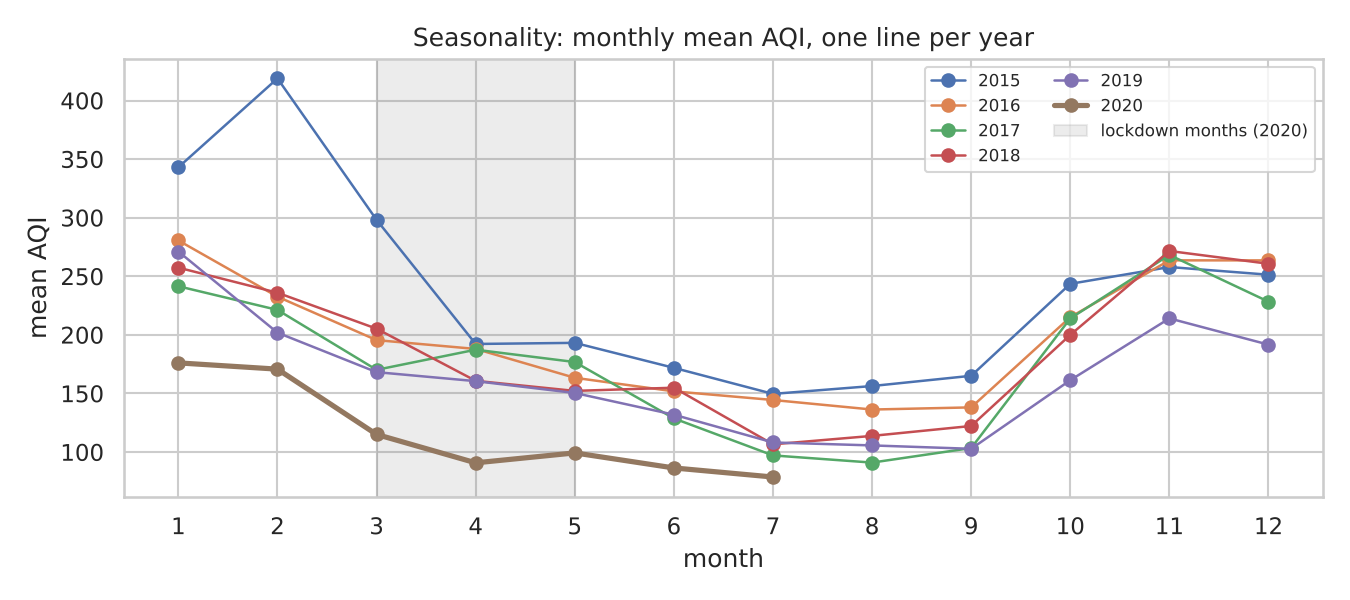
\includegraphics[width=\linewidth]{figures/03_aqi_monthly_by_year.png}\end{subfigure}\hfill
\begin{subfigure}{0.40\textwidth}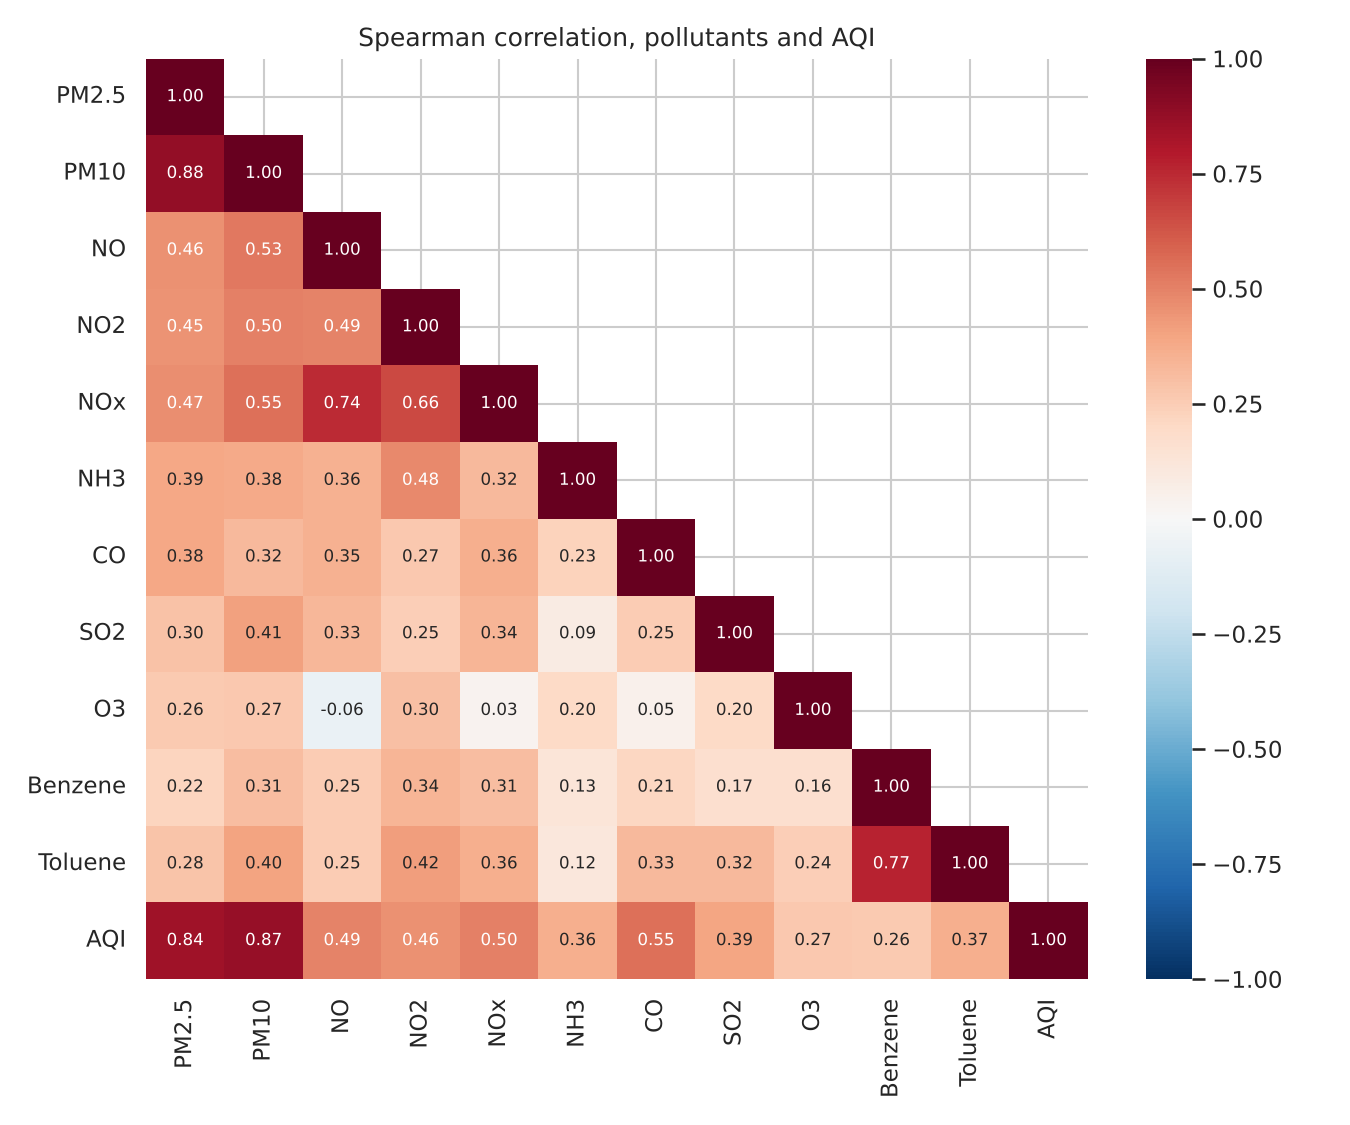
\includegraphics[width=\linewidth]{figures/03_corr_heatmap.png}\end{subfigure}
\caption{Left: winter peak and monsoon low every year, and the 2020 lockdown dip. Right: Spearman correlations; note the PM, NO and BTX blocks.}\vspace{-8pt}
\end{figure}

%-------------------------------------------------------------
\section{Preprocessing and feature engineering \quad {\small(\nb{04_preprocessing.ipynb}{04\_preprocessing})}}
\textbf{Split and leakage control.} Train 2015--18 (15{,}978 rows), validation 2019 (6{,}205), test Jan--Jun 2020 (3{,}111). The data is never shuffled across time. Modelling uses the 17 cities with at least 200 training AQI days. Every fitted quantity uses training rows only.

\textbf{Transform.} $z=(\log(1+x)-\mu_{\text{train}})/\sigma_{\text{train}}$. The log was applied because it reduced $|g_1|$ on train for all 11 pollutants.

\textbf{Imputation} (done in $z$-space):
(i) \emph{city median};
(ii) \emph{KNN}: $\hat z_{ij}=\frac1k\sum_{l\in N_k(i)} z_{lj}$, with neighbours found using the observed coordinates;
(iii) \emph{iterative low-rank SVD}: start with missing cells set to 0, then repeat $Z=U\Sigma V^\top$, $\hat Z=U_r\Sigma_rV_r^\top$, $Z_{\Omega^c}\leftarrow\hat Z_{\Omega^c}$ until convergence. A new row is filled by solving $\min_c\|z_o-V_{r,o}c\|^2+\lambda\|c\|^2$ over its observed entries $o$ and setting $z_m=V_{r,m}c$;
(iv) \emph{city-centred} versions: subtract the city median, impute the residual with (ii) or (iii), then add the median back.
To compare them, we hid 10\% of the observed validation values and measured $\text{RMSE}=\sqrt{\tfrac{1}{|H|}\sum_{H}(\hat z-z)^2}$ on those hidden cells:

\begin{table}[h]\centering\small\vspace{-4pt}
\setlength{\tabcolsep}{4pt}\begin{tabular}{lccccccc}\toprule
& city-KNN $k{=}80$ & city-KNN $k{=}40$ & city-SVD $r{=}1$ & KNN $k{=}40$ & SVD $r{=}1$ & city median & SVD $r{=}3$\\\midrule
RMSE (2 seeds) & \textbf{0.73 / 0.75} & 0.75 / 0.77 & 0.75 / 0.78 & 0.79 / 0.81 & 0.81 / 0.82 & 0.82 / 0.84 & 0.89 / 0.91\\\bottomrule
\end{tabular}\vspace{-6pt}
\end{table}
Most of the variation is \emph{between cities}. Plain KNN and SVD ignore this and barely beat the city median, and SVD with $r\ge3$ overfits. We chose city-centred KNN ($k{=}80$).

\textbf{Features.} The standardised pollutants; today's AQI (missing values filled with the city's training median, plus a missingness flag); one-day lags of PM2.5, PM10, NO$_2$ and AQI and a 7-day PM2.5 mean, all computed within each city; cyclic encodings $\sin(2\pi m/12),\cos(2\pi m/12)$ for month and the same for day of week; and city one-hot indicators (39 features in total). Targets: RQ1 uses $y=\log(1+\text{AQI}_t)$; RQ2 uses $y=\mathbb 1[\text{AQI}_{t+1}>200]$.

%-------------------------------------------------------------
\section{RQ1: what drives AQI? \quad {\small(\nb{05_rq1_regression.ipynb}{05\_rq1\_regression})}}
\textbf{Methods.} \emph{OLS} minimises $\|y-X\beta\|^2$, which gives $\hat\beta=(X^\top X)^{-1}X^\top y$ with $\operatorname{Var}(\hat\beta)=\sigma^2(X^\top X)^{-1}$. Collinearity is measured by $\text{VIF}_j=1/(1-R_j^2)$. \emph{PCR} regresses $y$ on the first $k$ principal-component scores, with $k$ chosen by 5-fold \texttt{TimeSeriesSplit} on train. \emph{KNN}, a \emph{random forest} (bagged CART trees with random feature subsets) and an \emph{MLP} (ReLU activations, Adam, L2 penalty) were tuned on validation. Metrics are computed on the AQI scale: RMSE, MAE and $R^2=1-\text{SS}_{\text{res}}/\text{SS}_{\text{tot}}$.

\begin{table}[h]\centering\small\vspace{-4pt}
\begin{tabular}{lccccc|lcc}\toprule
Model & Val RMSE & Test RMSE & Test MAE & Test $R^2$ & $R^2$ no lockdown & \multicolumn{3}{c}{Tomorrow's AQI (test)}\\\midrule
MLR & 59.2 & 35.7 & 22.4 & 0.844 & 0.860 & & RMSE & $R^2$\\
PCR ($k{=}10$) & 58.8 & 35.3 & 22.3 & 0.847 & 0.863 & Persistence & 47.7 & 0.717\\
KNN ($k{=}10$) & 54.3 & 36.2 & 22.0 & 0.839 & 0.851 & MLR & 41.5 & 0.786\\
Random forest & \textbf{49.5} & \textbf{29.5} & \textbf{17.1} & \textbf{0.894} & \textbf{0.909} & RF & \textbf{38.1} & \textbf{0.820}\\
ANN (64) & 51.4 & 33.0 & 19.9 & 0.866 & 0.886 & & &\\\bottomrule
\end{tabular}\vspace{-6pt}
\end{table}

\textbf{Results.}
\begin{itemize}
\item \textbf{Linear vs non-linear.} AQI is $\max_p I_p(c_p)$, where $I_p$ is a piecewise-linear sub-index of the concentration $c_p$. It is therefore non-linear in the pollutants, and the random forest reduces RMSE by 17\% compared with MLR.
\item \textbf{Collinearity.} All VIFs are below 2.7, so collinearity is milder than the raw $\rho$ suggests (many PM10 values are imputed, which weakens the PM2.5--PM10 link). Cross-validation picks $k=10$ of 11 components, and PCR $\approx$ MLR. With $n\gg p$, collinearity affects how stable individual coefficients are, not prediction accuracy.
\item \textbf{Drivers.} The standardised OLS coefficients are PM2.5 0.36, CO 0.27, PM10 0.16, and all others below 0.05. The random forest's permutation importance gives the same ranking (0.66, 0.36, 0.13).
\item \textbf{Ahmedabad check.} Without Ahmedabad, CO's coefficient \emph{halves} (0.27 $\to$ 0.135), so the CO effect comes mostly from one suspect sensor.
\item \textbf{Binding pollutant.} We recomputed the CPCB sub-indices $I_p=I_{lo}+\frac{I_{hi}-I_{lo}}{B_{hi}-B_{lo}}(c_p-B_{lo})$ from the daily values. These match the dataset's AQI with $r=0.88$, and the same bucket on 70\% of days. $\arg\max_p I_p$ is PM2.5 on 63\% of winter days, while PM10 dominates in summer (48\%). On unhealthy days PM2.5 binds in almost every city (Lucknow 99\%, Kolkata 99\%, Gurugram 94\%, Delhi 71\%); the exceptions are Ahmedabad (CO) and Talcher and Jorapokhar (PM10).
\item \textbf{Circularity.} Same-day $R^2$ is partly circular, because AQI is a function of the pollutants. The non-circular task (tomorrow's AQI, table right) still beats persistence.
\end{itemize}

%-------------------------------------------------------------
\section{RQ2: predicting tomorrow's unhealthy day \quad {\small(\nb{06_rq2_classification.ipynb}{06\_rq2\_classification})}}
\textbf{Methods.} \emph{Logistic regression} models $p_i=\sigma(\beta_0+x_i^\top\beta)$ and minimises the class-weighted, L2-penalised log-loss $-\sum_i w_{y_i}[y_i\log p_i+(1-y_i)\log(1-p_i)]+\tfrac{1}{2C}\|\beta\|^2$, with weights $w_c=n/(2n_c)$. $e^{\beta_j}$ is the odds ratio for a one-standard-deviation increase in feature $j$. \emph{LDA} assumes Gaussian classes with a shared covariance $\Sigma$, which gives the linear rule $\delta_c(x)=x^\top\Sigma^{-1}\mu_c-\tfrac12\mu_c^\top\Sigma^{-1}\mu_c+\log\pi_c$ ($\Sigma$ shrunk with Ledoit--Wolf). We also fit a \emph{decision tree} (Gini impurity $1-\sum_c p_c^2$), a \emph{random forest}, \emph{KNN} and an \emph{MLP}. Each model was tuned by validation ROC-AUC $=P(s(x^+)>s(x^-))$. The decision threshold maximises $F_\beta=(1+\beta^2)PR/(\beta^2P+R)$ with $\beta=2$ on validation, since a missed unhealthy day costs more than a false alarm. Test is evaluated once.

\begin{table}[h]\centering\footnotesize\setlength{\tabcolsep}{3.5pt}\vspace{-4pt}
\begin{tabular}{lccccc|lccccc}\toprule
Model & AUC & PR-AUC & Prec. & Rec. & $F_2$ & Model & AUC & PR-AUC & Prec. & Rec. & $F_2$\\\midrule
Majority class & 0.500 & 0.122 & 0 & 0 & 0 & LDA & 0.971 & 0.859 & 0.550 & 0.936 & 0.821\\
Persistence & 0.963 & 0.811 & 0.736 & 0.740 & 0.740 & Tree (depth 4) & 0.960 & 0.823 & 0.657 & 0.906 & 0.842\\
AQI$_t\ge$160 (tuned) & 0.963 & 0.811 & 0.567 & 0.906 & 0.809 & \textbf{Random forest} & \textbf{0.976} & 0.872 & 0.647 & 0.920 & \textbf{0.848}\\
Logistic regr. & 0.975 & 0.876 & 0.594 & 0.934 & 0.838 & KNN ($k$=61) & 0.950 & 0.783 & 0.420 & 0.914 & 0.740\\
& & & & & & ANN (64) & 0.974 & \textbf{0.879} & 0.622 & 0.931 & 0.847\\\bottomrule
\end{tabular}
\caption{Test set 2020 (2{,}963 days, 12.2\% positive). The majority class reaches 87.8\% accuracy with zero recall.}\vspace{-6pt}
\end{table}

\begin{figure}[h]\centering\vspace{-6pt}
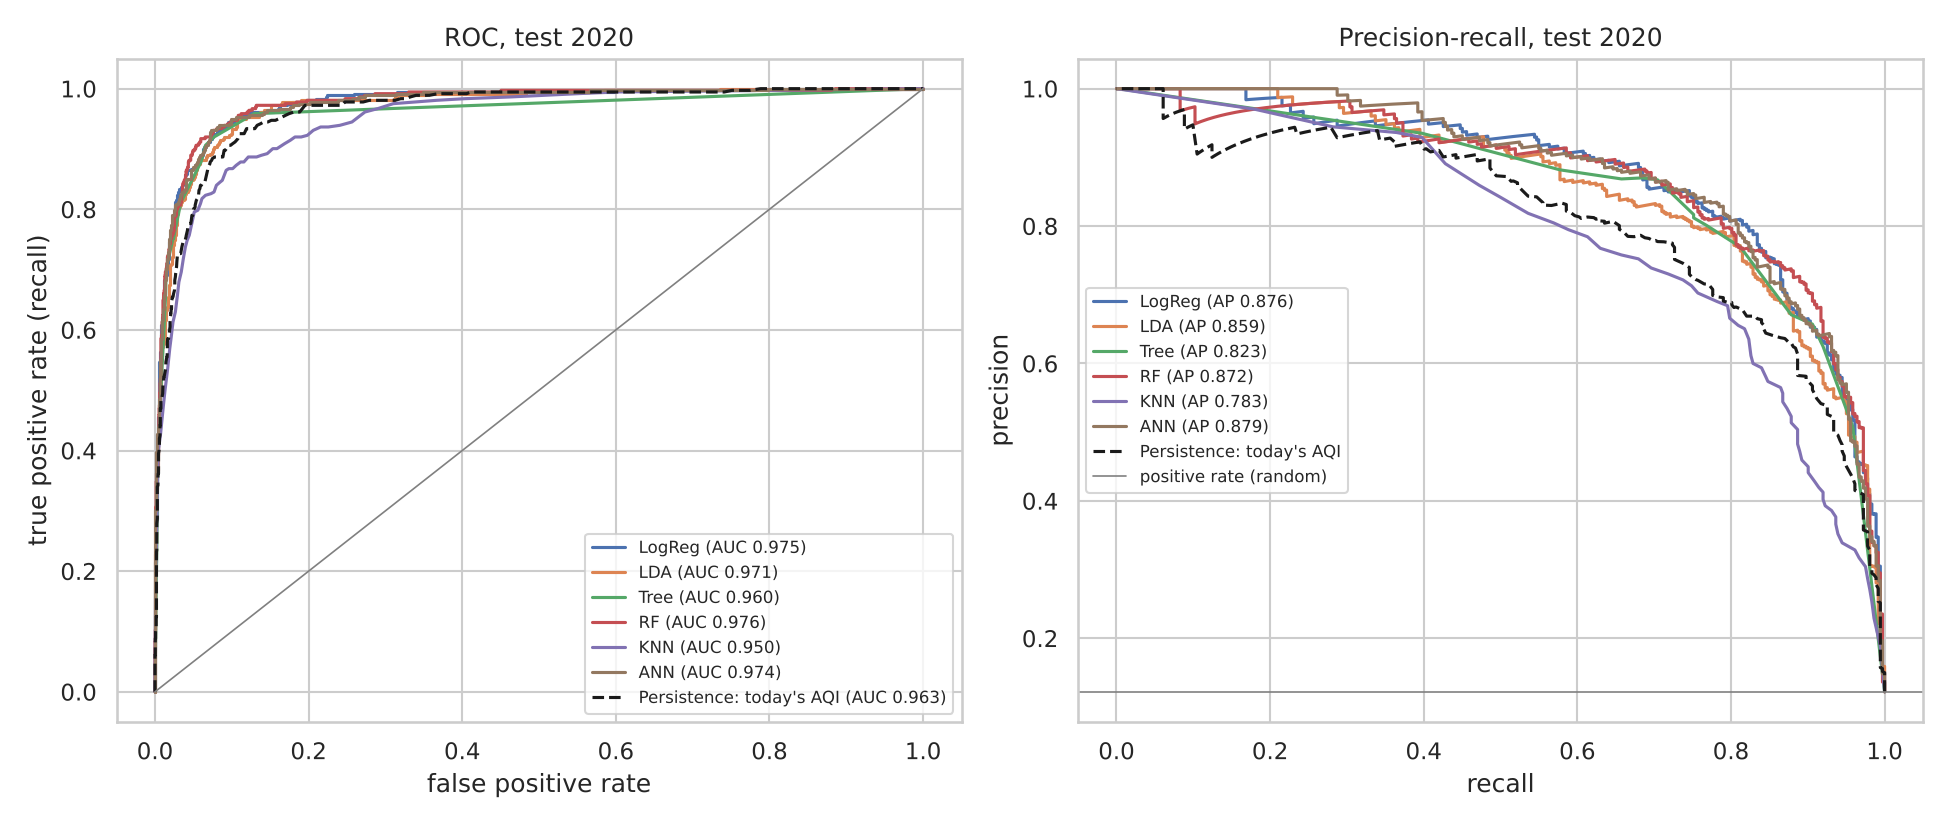
\includegraphics[width=0.78\textwidth]{figures/06_roc_pr.png}
\caption{ROC and precision--recall curves on the 2020 test set. The dashed curve uses today's AQI as the score.}\vspace{-8pt}
\end{figure}

\textbf{Results.}
\begin{itemize}
\item \textbf{Fair baseline.} The models are tuned, so the honest baseline is today's AQI with its own threshold tuned on validation. Against it, the best models gain $+0.013$ AUC, $+0.06$ PR-AUC and $+0.04$ $F_2$. The gain is real but modest; most of the signal is today's AQI.
\item \textbf{Transitions.} On transition days (healthy $\to$ unhealthy, 297 days), recall is 0\% for persistence, 71\% for the tuned baseline, 75\% for the random forest and 81\% for logistic regression. The cost is false alarms on 91--96\% of the days after an episode ends.
\item \textbf{Interpretation.} The depth-3 tree reads: alarm if AQI$_t>185$, or if PM2.5$_t>84\,\mu$g/m$^3$ (stronger when the 7-day mean is $>89$). Logistic odds ratios: AQI$_t$ 6.7, PM2.5$_t$ 6.1, PM10$_t$ 2.8, AQI$_{t-1}$ 2.5; PM2.5$_{t-1}$ 0.36 (with today fixed, rising pollution raises the risk).
\item \textbf{Robustness.} Without Ahmedabad, AUC is unchanged (0.975 / 0.976). Oversampling gives the same AUC as class weights (0.975). Without the lockdown months, $F_2$ rises to 0.89.
\end{itemize}

%-------------------------------------------------------------
\section{RQ3: city pollution profiles \quad {\small(\nb{07_rq3_profiles.ipynb}{07\_rq3\_profiles})}}
\textbf{Data matrix.} 19 cities with at least a full year of data, excluding the lockdown months. Each city is described by 16 features: the median and 90th percentile (log scale) of PM2.5, NO, NO$_2$, CO, SO$_2$ and O$_3$; the shares of days Good/Satisfactory, Moderate and Poor+; and $\log(\text{PM2.5}_{\text{winter}}/\text{PM2.5}_{\text{monsoon}})$. The matrix is standardised.

\textbf{PCA via SVD.} For the centred matrix $X=U\Sigma V^\top$, the covariance is $S=\frac{X^\top X}{n-1}=V\frac{\Sigma^2}{n-1}V^\top$. So the loadings are the columns of $V$, the eigenvalues are $\lambda_j=\sigma_j^2/(n-1)$, and the scores are $T=XV=U\Sigma$. We verified numerically that scikit-learn's PCA and \texttt{numpy.linalg.svd} agree up to sign. PC1, PC2 and PC3 explain 42\%, 18\% and 14\%, and 4 PCs explain 80\%.
\begin{itemize}
\item \textbf{PC1 is overall pollution:} PM2.5, NO, CO, SO$_2$ and the Poor+ share load positively (0.37), and the Good share negatively ($-0.33$).
\item \textbf{PC2 contrasts NO$_2$ and O$_3$} (traffic and photochemistry, 0.37--0.50) with PM, NO and winter seasonality.
\item \textbf{PC3 is CO and SO$_2$} (industrial combustion).
\end{itemize}

\textbf{Clustering.} k-means minimises $J=\sum_{k=1}^K\sum_{i\in C_k}\|x_i-\mu_k\|^2$ by alternating two steps (assign each point to its nearest $\mu_k$; recompute each $\mu_k$ as its cluster mean), using 50 random starts on the first 4 PC scores. $K$ was chosen with the silhouette $s_i=\frac{b_i-a_i}{\max(a_i,b_i)}$, which is highest at $K=4$ (0.38). Ward hierarchical clustering agrees with an adjusted Rand index (ARI) of 0.83.

\begin{figure}[h]\centering\vspace{-6pt}
\begin{minipage}{0.44\textwidth}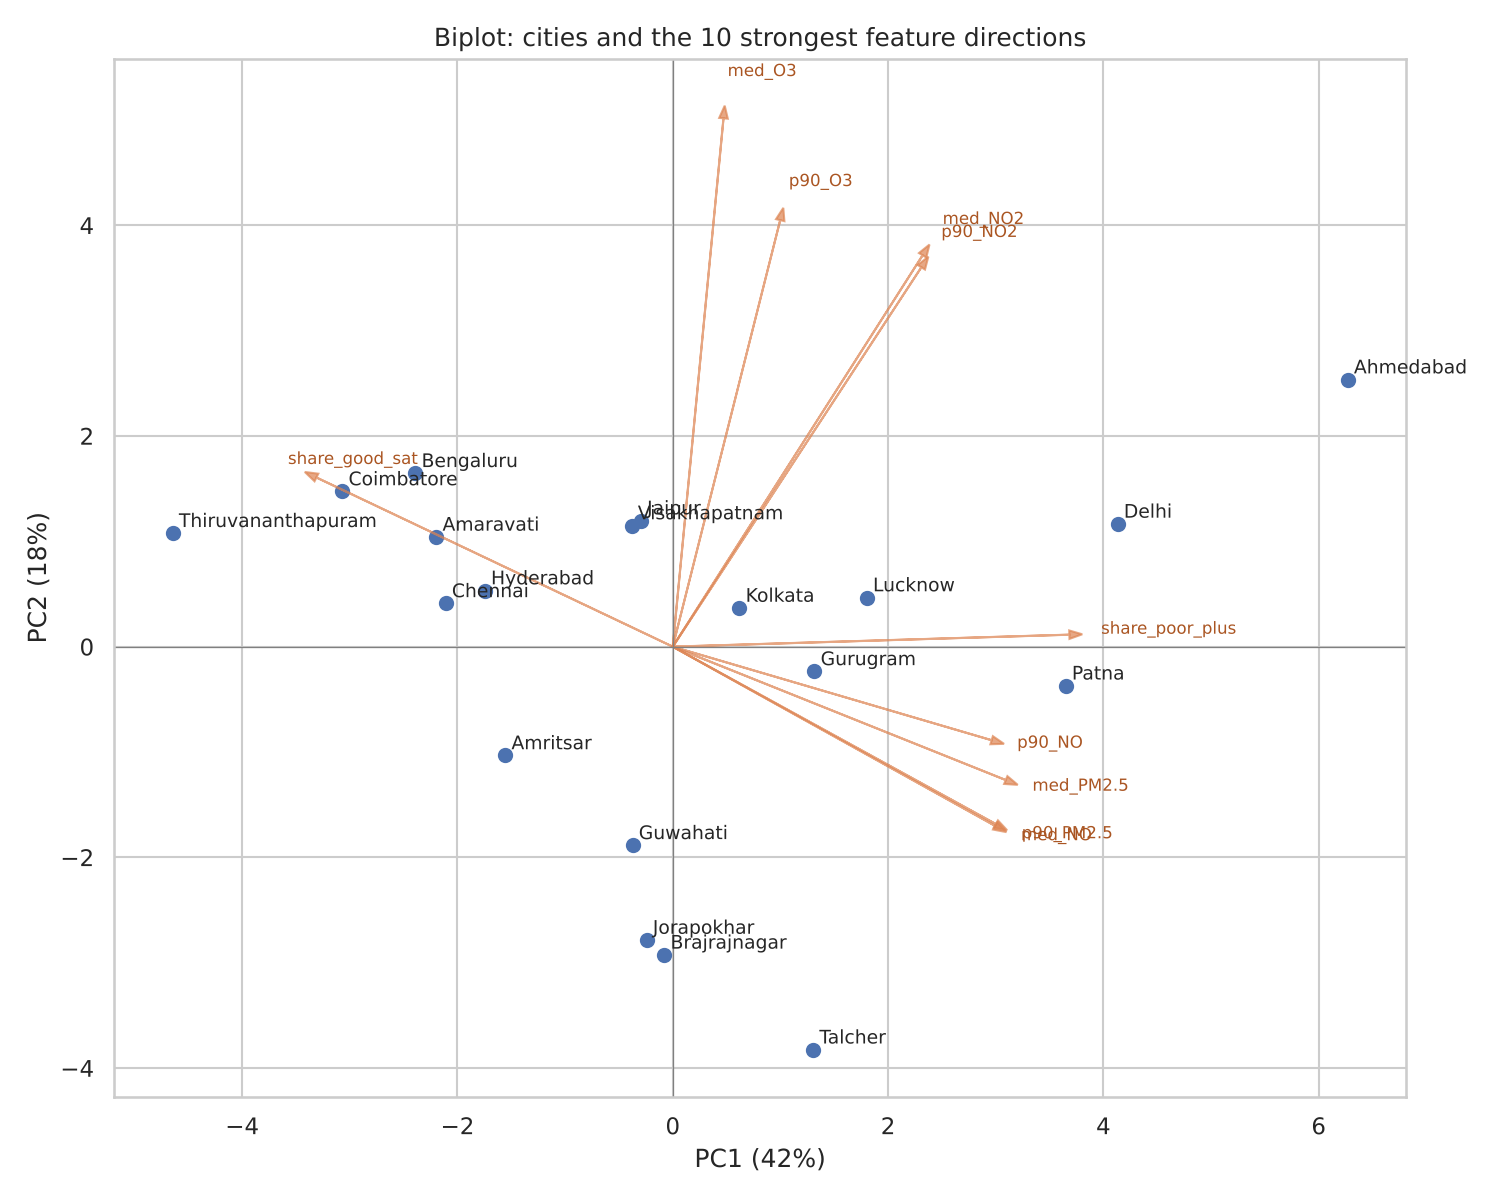
\includegraphics[width=\linewidth]{figures/07_biplot.png}\end{minipage}\hfill
\begin{minipage}{0.54\textwidth}\footnotesize\setlength{\tabcolsep}{3pt}
\begin{tabular}{>{\raggedright\arraybackslash}p{4.5cm}>{\raggedright\arraybackslash}p{4.5cm}}\toprule
Cluster & Profile\\\midrule
Indo-Gangetic: Delhi, Gurugram, Lucknow, Patna, Kolkata & PM2.5 86\,$\mu$g/m$^3$, 52\% of days Poor+, winter/monsoon PM2.5 $\approx4\times$\\
Cleaner (9 cities): Chennai, Bengaluru, Hyderabad, Coimbatore, Jaipur, \dots & PM2.5 38, 6\% Poor+\\
Eastern industrial: Talcher, Brajrajnagar, Jorapokhar, Guwahati & low NO$_2$/O$_3$, PM2.5 55, winter $4.2\times$\\
Ahmedabad (alone) & CO 17\,mg/m$^3$, SO$_2$ 48, 86\% Poor+\\\bottomrule
\end{tabular}\end{minipage}
\caption{PCA biplot of the 19 cities, and the k-means profiles ($K=4$).}\vspace{-8pt}
\end{figure}

\textbf{Stability and geography.} Resampling days 50 times (bootstrap) gives a mean ARI of 0.96 (minimum 0.51). Changing $K$ to 3 or 5 gives ARI 0.75 and 0.80. Without Ahmedabad the ARI is 0.68, but the Indo-Gangetic cluster is unchanged. The clusters largely follow geography: the whole first cluster lies on the Indo-Gangetic Plain, and the industrial cluster contains the Odisha and Jharkhand coal belt. The misfits are Amritsar and Jaipur (northern but in the cleaner cluster) and Guwahati.

%-------------------------------------------------------------
\section{Discussion: research questions answered}
\textbf{RQ1.} \textbf{PM2.5 is the dominant driver}: it is the binding pollutant on most unhealthy days, especially in winter and the post-monsoon season. CO matters mainly through Ahmedabad's suspect sensor. AQI is predictable from same-day pollutants ($R^2=0.89$, RF), but that is partly by construction. Tomorrow's AQI is predictable with $R^2=0.82$.

\textbf{RQ2.} \textbf{Yes.} Unhealthy days can be flagged one day ahead with ROC-AUC 0.976 and recall 0.92. However, a tuned rule ``warn if today's AQI $\ge160$'' already reaches AUC 0.963 and recall 0.91. The models add a modest, consistent gain, mostly by catching rising-pollution transitions.

\textbf{RQ3.} \textbf{Yes, four stable profiles} on about three latent factors: overall level, traffic and photochemical gases vs particulate seasonality, and industrial combustion. The three analyses agree: the PM-led PC1 matches the RQ1 drivers, and the Indo-Gangetic cluster holds most of the RQ2 positives. The practical priority is the Indo-Gangetic cities from October to February.

\textbf{Limitations and bias.}
\begin{itemize}
\item Imputation error is still 0.73\,SD, and pollutants a city never measured are borrowed from other cities.
\item Station coverage is uneven: 8 cities are excluded from modelling.
\item There is no weather data (wind, rain, mixing height), which limits day-ahead skill.
\item The 2020 test year is atypical (lockdown; the positive rate halves), and precision depends on the positive rate.
\item Some sensors are suspect: Ahmedabad CO, exact zeros, Talcher O$_3$.
\item With 19 cities, the clustering is descriptive.
\end{itemize}

\textbf{Future work.} Add ERA5 meteorology; use time-series and boosted models; forecast 2--3 days ahead; build station-level models; and recompute the official AQI from hourly data.

\section{Learnings and conclusion}
\begin{itemize}
\item \textbf{Order of operations prevents leakage:} split by time first, then fit transforms and imputers on train only.
\item \textbf{A metric only means something next to an honest baseline.} Tuning the threshold for the models but not the baseline would have overstated the gain several-fold. Accuracy was useless under imbalance.
\item \textbf{Know how the target is built.} Because AQI $=\max_p I_p$, same-day regression is circular. The binding-pollutant analysis turned that into an interpretable result.
\item \textbf{Collinearity hurts interpretation more than prediction,} which is why PCR $\approx$ MLR.
\item \textbf{PCA is the SVD of the centred data matrix,} and low-rank structure can also be used to impute missing values.
\item \textbf{Inspect anomalies before modelling:} one suspicious sensor (Ahmedabad CO) shifted a regression coefficient by a factor of 2 and formed its own cluster.
\end{itemize}

In conclusion, fine particulate pollution, concentrated on the Indo-Gangetic Plain in winter, drives unhealthy air in Indian cities. Next-day warnings are feasible with simple, interpretable models, and cities group into a few stable, geographically meaningful profiles.

\vspace{2pt}
\begin{table}[h]\centering\small\vspace{-6pt}
\begin{tabular}{lll}\toprule
Member & Role & Contribution\\\midrule
Arahana Garg (2024MCB1261) & Data cleaning, EDA & Steps 1--3, notebooks 02--03\\
Kushagra Gupta (2024MCB1299) & Regression, PCR, PCA/SVD & Step 5, imputation (Step 4)\\
Saurabh Sharma (2024MCB1311) & Classification, ROC analysis & Step 6, feature engineering\\
Manish Kumar Chatakunda (2024MCB1302) & Clustering, report & Step 7, report and documentation\\\bottomrule
\end{tabular}
\caption{Member roles and contributions.}\vspace{-8pt}
\end{table}

{\small\textbf{References.}
[1]~R.~Rao, \emph{Air Quality Data in India (2015--2020)}, Kaggle.
[2]~CPCB, \emph{National Air Quality Index}, 2014.
[3]~Hastie, Tibshirani, Friedman, \emph{The Elements of Statistical Learning}, 2nd ed., Springer, 2009.
[4]~Pedregosa et al., Scikit-learn, \emph{JMLR} 12, 2011.}
\end{document}
